\documentclass{article}

\usepackage[utf8]{inputenc}
\usepackage[T1]{fontenc}
\usepackage[spanish]{babel}
\usepackage{times}
\usepackage{wrapfig}
\usepackage{lmodern}
\usepackage{mathtools}
\usepackage{graphicx}
\usepackage{color}
\usepackage{hyperref}
\usepackage{fancyhdr,lipsum}


\hypersetup{
    colorlinks=true, %set true if you want colored links
    linktoc=all,     %set to all if you want both sections and subsections linked
    linkcolor=blue,  %choose some color if you want links to stand out
}
\urlstyle{same}

\title{IntelliJ-IDEA\\\textbf{DOCUMENTACIÓN}}
\author{Miguel Ángel García, Francisco Moreno, Ángel Rabasco\\ y \\Antonio Muñoz}
\date{12 de Noviembre de 2020}



\begin{document}
  \maketitle
    \pagenumbering{gobble}
      \pagestyle{fancy}

      \begin{figure}[b]
        \centering
        
\includegraphics[scale = 0.5]{img/logo.png}
      \end{figure}
  
  \newpage
    \tableofcontents
      \lhead[Intellij-IDEA]{Intellij-IDEA}
        \lfoot[IES Francisco De Los Rios]{IES Francisco De Los Rios}

  \newpage
    \pagenumbering{arabic}
    \section{Introducción}
      En esta tarea vamos a tener que instalar, probar, familiarizarnos y documentar el uso de un \textit{IDE} de desarrollo para el lenguaje \textbf{\textit{JAVA}}, en el caso de nuestro grupo 
      hemos decidio usar el \textit{IDE \textbf{Intellij-IDEA}}. 
      \\\\
      \begin{minipage}{0.5\textwidth}
        \href{https://www.jetbrains.com/es-es/idea/}{Intellij IDEA} es un entorno de desarrollo integrado(IDE) para el desarrollo de programas informáticos. Es desarrollado por \textbf{JetBrains} 
        (anteriormente llamada IntelliJ), y está disponible en dos versiones, una gratuita para la comunidad y otra edición comercial.
      \end{minipage}
      \begin{minipage}{\textwidth}
        
\includegraphics[scale=0.15]{img/logo2.png}
      \end{minipage}
      \\
      Para el desarrollado de esta tarea, usaremos una metodología \textbf{SCRUM}, que es una de las metodologías de desarrollo ágil más usadas en la actualidad, dividimos el trabajo en diferentes
      tramos llamados \textbf{SPRINT}.
      \\\\
      \begin{figure}[h]
        \centering
        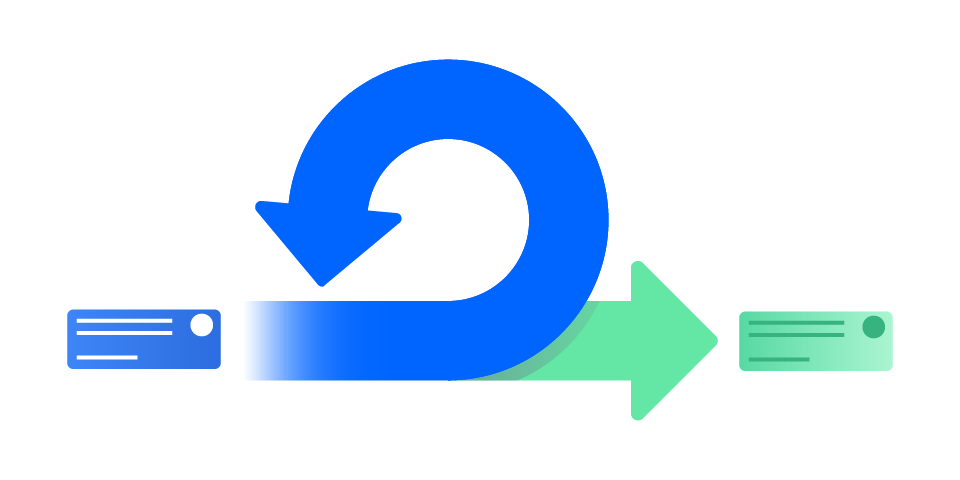
\includegraphics[scale = 0.5]{img/sprint.png}
      \end{figure}

  \newpage
    \section{Sprint 1}
      \subsection{Reunión de planificación de Sprint}
        En la planificación del primer sprint estuvimos leyendo e intercambiando opiniones sobre el Sprint Backlog que se nos disponía en la práctica, para afrontar la tarea de una forma 
        precisa y segura.
        \\
        \subsection{Sprint Backlog}
          \begin{figure}[h]
            \centering
            
\includegraphics[scale = 0.5]{img/backlog.png}
          \end{figure}
        
          \begin{itemize}
            \item Instalar entornos de desarrollo, propietarios y libres.
            \item Añadir y eliminar módulos en el entorno de desarrollo.
            \item Personalizar y automatizar el entorno de desarrollo
            \item Configurar el sistema de actualización del entorno de desarrollo.
            \item Generar ejecutables a partir de código fuente de diferentes lenguajes en un mismo entorno de desarrollo.
            \item Identificar las características comunes y específicas de diversos entornos de desarrollo.
            \item Identificar las funciones más usuales de las herramientas CASE para el desarrollo, prueba y documentación de código.
          \end{itemize}
        
        Después de un tiempo debatiendo, acordamos que lo mas sensato y lógico es que todos los miembros del grupo nos instalemos el IDE, para tener una experienza propia que nos ayuda a la hora
        de realizar cada una de las etapas del \textit{Sprint Backlog}, puesto que 4 mentes trabajan mejor que 1. Pero hemos definido una serie de pautas a seguir, para que todos sigamos un 
        mismo guión.
        \\
        \subsection{Analisis del Sprint Backlog}
        \begin{itemize}
          \item Vamos a añadir los módulos necesarios para facilitarnos el uso del IDE.
          \item También vamos a personalizarlo para que nos sea mas práctico y como de usar.
          \item También vamos a ver como se actualiza para tenerlo en su última versión.
          \item Usaremos varios lenguajes de programación para ver la versatilidad del entorno de desarrollo y generaremos ejecutables.
          \item Vamos a listar una serie de ventajas y desventajas del entorno de desarrollo.
          \item También identificaremos las funciones mas comunes de las herramientas CASE.
        \end{itemize}
        
        En el siguiente punto tuvimos una \textbf{lluvia de ideas}.
        
        \subsection{Lluvia de Ideas}
          \begin{figure}[h]
            \centering
            
\includegraphics[scale=0.5]{img/storm.jpg}
          \end{figure}
          Para saber que \textit{"producto"} entregar finalmente, entre las muchas opciones que barajamos en la reunión las más significativas 
          fueron las siguientes.
          \begin{itemize}
            \item Tenemos pensado hacer un video tutorial para explicar el uso y funcionamiento del entorno de desarrollo.
            \item Usar un tablero de \href{https://trello.com}{Trello} para repartirnos las tareas.
            \item Estamos barajando exponerlo en clase.
            \item Estamos barajando exponerlo en clase.
          \end{itemize}

        \subsection{Definimos el producto a entregar}
           Después de que este punto del sprint fuera debatido en la reunión con el personal, decidimos tomar como válida la opción de crear un video tutorial que nos muestre como usar el IDE 
           sus funcionalidades y su uso, pues se hace el aprendizaje más ameno, pero también decidimos realizar una documentación del IDE, para aportar algoa la comunidad, puesto que siempre 
           es de buen uso la documentación de cualquier herramienta.

        \subsection{Lista de lo que sabemos sobre IntelliJ IDEA}
          NADA XD
        \subsection{Lista de lo que NO sabemos sobre IntelliJ IDEA}
          \begin{itemize}
            \item Chain completion
            \item Static member completion
            \item Language injection
            \item Smart refactoring
            \item Cross-language refactoring
            \item Polyglot
          \end{itemize}
        

\end{document}